\sys's design includes a novel task scheduler. It uses efficient, energy-aware task coalescing to amortize static task overheads, and a timer-based task-splitting mechanism to avoid non-termination of tasks too long for a device's energy buffer. 

\subsection{Task Coalescing}
\label{sec:task_coalescing}

When a device's buffered energy is sufficient to run multiple tasks without a power failure, committing state after each task is unnecessary overhead. \sys reduces this overhead by coalescing a sequence of tasks and deferring commit
operations for all tasks to the end of the sequence. In general, committing involves moving state manipulated by a task into its permanent location in non-volatile memory. In particular, \sys's commit procedure copies dirty pages of memory that a task updated from fast, volatile working memory to slower, non-volatile main memory. We defer the details of paging privatization and commit to Section~\ref{sec:memory_virtulaization}.
An effective coalescing strategy must be {\em aggressive} enough, attempting to coalesce a large number of tasks to amortize commit overhead.
However, it must also be  {\em conservative} enough, coalescing only as many tasks as will execute to completion given certain energy conditions, reducing the risk of re-execution penalty for long coalesced tasks.

\subsubsection{Generic Design of Task Coalescing Strategies}
\label{subsec:coalescingGeneral}

% Coalescing has a double benefit. First, coalescing reduces the total number of relatively high-latency, high-energy non-volatile memory accesses because tasks primarily access variables in relatively low-latency, low-energy volatile memory. Second, coalescing eliminates the unnecessary instructions that implement task commit, which constitute a substantial run-time overhead, as our measurements in Section~\ref{sec:evaluation} show.

\begin{algorithm}[t]
	\caption{Coalescing}
	\label{algo:genCoalescing}
	\scriptsize
	\begin{algorithmic}[1]
        \State $C \leftarrow $ \Call{$f_\text{reboot}$}{$z$} \Comment{Update coalescing target by reboot update function}
        \State $H \gets 0$ \Comment{Initialize history}
        \While{$\texttt{true}$}       
	        \State $ i \gets 0$
	        %
	        \While{$ i <= C$}
		        \State \Call{execute\_task}{$T_\texttt{i}$}
		        \State $W \leftarrow $ \Call{$f_\text{weight}$}{$T_\text{i}$} \Comment{Assign new task-dependent weight}
		        \State $i \gets i + W$
				\State $H \gets H + W$
	        \EndWhile
	        %
	        \State \Call{commit\_to\_fram}{\null}
                \State $C \leftarrow $ \Call{$f_\text{commit}$}{$C$} \Comment{Update coalescing target by commit update function}
        \EndWhile
	\end{algorithmic}
\end{algorithm}

Algorithm~\ref{algo:genCoalescing} shows the general structure of a coalescing strategy. In the algorithm, $C$ (coalescing target) is total number of static tasks that \sys will next attempt to coalesce. $T_\text{i}$ is the $i$th task executed since the last power failure. $H$ (history) is the total number of tasks executed since the last power failure. $W_\text{i}$ is the {\em weight} of a task. A task's weight is an arbitrary quantity associated with the task that represents its cost in time or energy to execute. Different coalescing strategies may apply different weights to a task, e.g., $W_\text{i} = 1\ \forall i$, or $W_\text{i} = \alpha E(T_\text{i})$ where $E(T_\text{i})$ is the average execution time of $T_\text{i}$ and $\alpha$ is a constant.
% For example, a uniform weighting scheme sets the weight of each task to one, making them all effectively equal in cost to the coalescing algorithm.  A different policy might use a weighting scheme that sets a task's weight equal to its run time relative to the task that executes for the shortest duration, which has unity weight. 

\subsubsection{Example Task Coalescing Strategies}
\label{subsec:coalescingStrategies}

Different coalescing strategies adhere mainly to the template in Algorithm~\ref{algo:genCoalescing}, varying in only a few {\em characteristic operations} that the algorithm leaves deliberately abstract. The reboot update function, $f_\text{reboot}$, updates $C$, the coalescing target, after a reboot. The weight lookup function $f_\text{weight}$ returns a task's weight. The commit update function $f_\text{commit}$ updates $C$ after a successful commit. The following paragraphs detail three coalescing strategies that we developed for \sys, albeit not the only possible. In fact, \sys \emph{allows programmers to design their own strategy} to implement and link against \sys's task scheduler. 

\paragraph{Energy-Oblivious Coalescing.}
\label{subsec:energyBlind}
 
A very simple {\em energy-oblivious} (EO) coalescing strategy treats all tasks as having unity weight and varies the size of the coalescing target linearly. In such a scheme, the number of tasks to coalesce, $C$, increases by a constant $x$ when a coalesced sequence of tasks commits, and decreases by the same constant $x$ when a coalesced sequence of tasks fails to complete, i.e., after a power failure. The characteristic operations of EO are
%
\begin{equation}
	\begin{split}
		f_\text{reboot}(C) & = C - x, \\
		f_\text{weight}(T_\text{i}) & =  1, \\
		f_\text{commit}(C) & = C + x.
	\end{split}
	\label{eq:eo}
\end{equation}
%
EO reacts slowly to the variation in the energy required to execute different tasks and to the variation in the effective quantum of energy available to the device. With the successful commit of each coalesced task sequence, $C$ increases. Eventually, the target may be too high and only a coalesced task composed of a few units will commit without interruption by a power failure. The strategy then linearly decreases $C$, eventually reaching a value that allows completion. A key limitation of this algorithm lies in the equality of the target decrease in $f_\text{reboot}$ and the increase in $f_\text{commit}$. Let us assume $x=1$. If, after $k$ successful commits, the target must decrease to its original value $C-k$ due to an energy drop, EO requires $k$ successive power failures, before being able to progress.

\paragraph{Energy-Guided Coalescing.}
\label{subsec:energyAware}

\begin{figure*}
    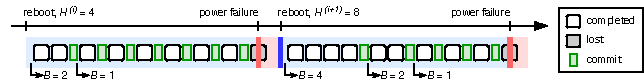
\includegraphics[width=\linewidth]{figures/hg-coal-horiz.pdf}
    \caption{EG coalescing sample execution across two power cycles. \emph{C}: coalescing target, \emph{H}: history.}
    \label{fig:hg-coal}
\end{figure*}

The \emph{Energy-Guided} (EG) coalescing strategy adapts its coalescing target more quickly, addressing a key limitation of the EO, to adhere to changes in energy conditions. It uses its recent execution history, H, to estimate energy availability and alters its target accordingly. The EG algorithm is characterized by the following functions
%
\begin{equation}
	\begin{split}
		 f_\text{reboot}(H) & = \lceil \rho H \rceil,\\
		 f_\text{weight}(T_\text{i}) & = 1, \\
		 f_\text{commit}(C) & = \lceil \gamma C \rceil,
	\end{split}
	\label{eq:eg}
\end{equation}
%
where $\rho, \gamma \in [0, 1]$. By relying on the history of execution EG eliminates the problem of frequent power failures on a single coalesced task. In fact, at each reboot, EG will {\em conservatively} try to coalesce only a fraction ($\rho$) of tasks that had successfully completed during the last power cycle.
% In fact EG can reduce its target to one from any coalesced target in at most two successive power failures. For instance, if the execution is interrupted after finishing a single task the history will be one ($H = 1$) and the target will be set to one also. While a history of $H$ suggests that there is sufficient energy to coalesce and successfully commit $H$ tasks (i.e., to set $C = H$). EG conservatively sets $C$ equal to half of $H$ moderating the risk of a very long coalesced task. We experimented with a range of fraction values, settling on one half as the default for EG, because one half had the highest performance.
Fig.~\ref{fig:hg-coal} illustrates a snapshot of the operation of EG, with $\rho = \gamma = 0.5$. The figure shows two power cycles following the $i$th, the latter having an execution history $H^{(i)} = 4$. Based on that, $C$ is initially set to two and then decreases to one. Once the value of $C$ reaches one, EG is expecting a power failure, justifying the conservative approach. After the reboot, EG uses the most recent history $H^{(i+1)} = 8$ to set $C = 4$ and continue execution.

\paragraph{Weighted Energy-Guided Coalescing.}
\label{subsec:energyTaskAware}

The \emph{Weighted Energy-Guided} (WEG) coalescing strategy accounts for non-uniform energy and time costs of a program's tasks when setting $C$. Each different task in the program consumes a different amount of energy to run to completion. The EO and EG coalescing strategies assume that each task has the same cost: for these strategies, $C$ simply corresponds to a target {\em count} of tasks to coalesce, regardless of the individual cost of each task. However, if one task executes for ten seconds and another executes for one second, counting tasks misjudges the amount of {\em work} in the coalesced tasks (and the history).
%
Instead, WEG associates a non-unity weight with each task in the program, and tracks the sum of the weights of tasks in a coalesced sequence. When the sum of weights reaches $C$, the target, WEG commits the coalesced task.
% WEG differs from EO and HG by explicitly accounting for the variation in energy cost of a program's tasks, eliminating the assumption that all tasks do the same work, which is a key limitation.
WEG is characterized the same way as EG (equation (\ref{eq:eg})), except that $f_\text{weight}(T_\text{i}) = W_\text{i}$.
%
% The effectiveness of the WEG hinges on correctly identifying the weight of each task, which WEG assumes is {\em statically} available. Profiling the time and energy cost of tasks in a program is a difficult, orthogonal problem~\cite{cleancut_2018,baghsorkhi_cgo_2018}. WEG could use the result of an arbitrarily sophisticated profiling procedure. To produce a concrete result in this paper, we give WEG access to a simple profile of task run time collected offline using a single fixed input. WEG stores the profile in a lookup table that maps a task's identifier to its weight, making the information available to \sys's scheduler at run time.
